\documentclass[10pt]{article}
	
\usepackage[margin=1in]{geometry}		% For setting margins
\usepackage{amsmath}				% For Math
\usepackage{fancyhdr}				% For fancy header/footer
\usepackage{graphicx}				% For including figure/image
\usepackage{float}
\usepackage{hyperref}
\usepackage{tabto}
\usepackage{cancel}					% To use the slash to cancel out stuff in work
% avoid all eq numbering via:
% \usepackage{mathtools}
% \mathtoolsset{showonlyrefs}

\usepackage{cite}
\usepackage{url}
\usepackage{amssymb}                % To include mathbb symbols
\usepackage{graphicx}               % In preamble
\newcommand{\mcG}{\mathcal{G}}
\newcommand{\mcU}{\mathcal{U}}
\newcommand{\mcV}{\mathcal{V}}


% Set up fancy header/footer
\pagestyle{fancy}
\fancyhead[LO,L]{Bionics and Wearable Robotics 0360108}
\fancyhead[CO,C]{Homework 2}
\fancyhead[RO,R]{\today}
\fancyfoot[LO,L]{}
\fancyfoot[CO,C]{\thepage}
\fancyfoot[RO,R]{}
\renewcommand{\headrulewidth}{0.1pt}
\renewcommand{\footrulewidth}{0.1pt}
% \renewcommand{\thesubsection}{(\roman{subsection})}
\renewcommand{\thesubsubsection}{(\roman{subsubsection})}

%%%%%%%%%%%%%%%%%%%%%%

\begin{document}
\begin{table}[h]
    \centering
    \begin{tabular}{l l l}
        \hline
        Name & ID & Email \\
        \hline
        Elad Siman Tov & - & elad.sim@campus.technion.ac.il \\
        \hline
        Eitan Gerber & - & eitangerber@campus.technion.ac.il \\
        \hline
    \end{tabular}
    \label{tab:personal_info}
\end{table}

% -------------------------------------- %
% -------------- NOTES ----------------- %
% -------------------------------------- %
\section{Gait Event Detection Method - \href{https://github.com/eladsimantov/Wearable-Robotics/blob/main/HW2/gaitEventDetector.ino}{Link To Code}}
To identify Heel Strike (HS) and Toe Off (TO) we placed the IMU on the ankle, and based the detection on two states logic with the two gait events to toggle between the states. Note that to toggle between states it is sufficient to use a single memory bit (such as HS) but we used both for clarity of our program. The states and their transitions are shown in the state diagram in Figure \ref{fig:stateDiagram}.
The default state is during stance ($\mathcal{ST}$), after HS triggers and before TO. The second state is swing ($\mathcal{SW}$), when the foot is above ground.  
At both gait events, we assumed that the acceleration will record a peak, so we added a threshold of 11.5 $m/s^2$ for entering swing and 11 $m/s^2$ to transition to stance. At HS, we assume that the foot angle is negative with respect to the ground (assuming positive for plantar-flexion) and at TO we assume a positive angle. In addition, we used the switching of signs of the angular velocities for the state transitions. Once each state is entered we added a delay of $\Delta T\ge150\,[ms]$ under which no transition can follow to avoid rapid state transitions. 
\begin{figure}[H]
    \centering
    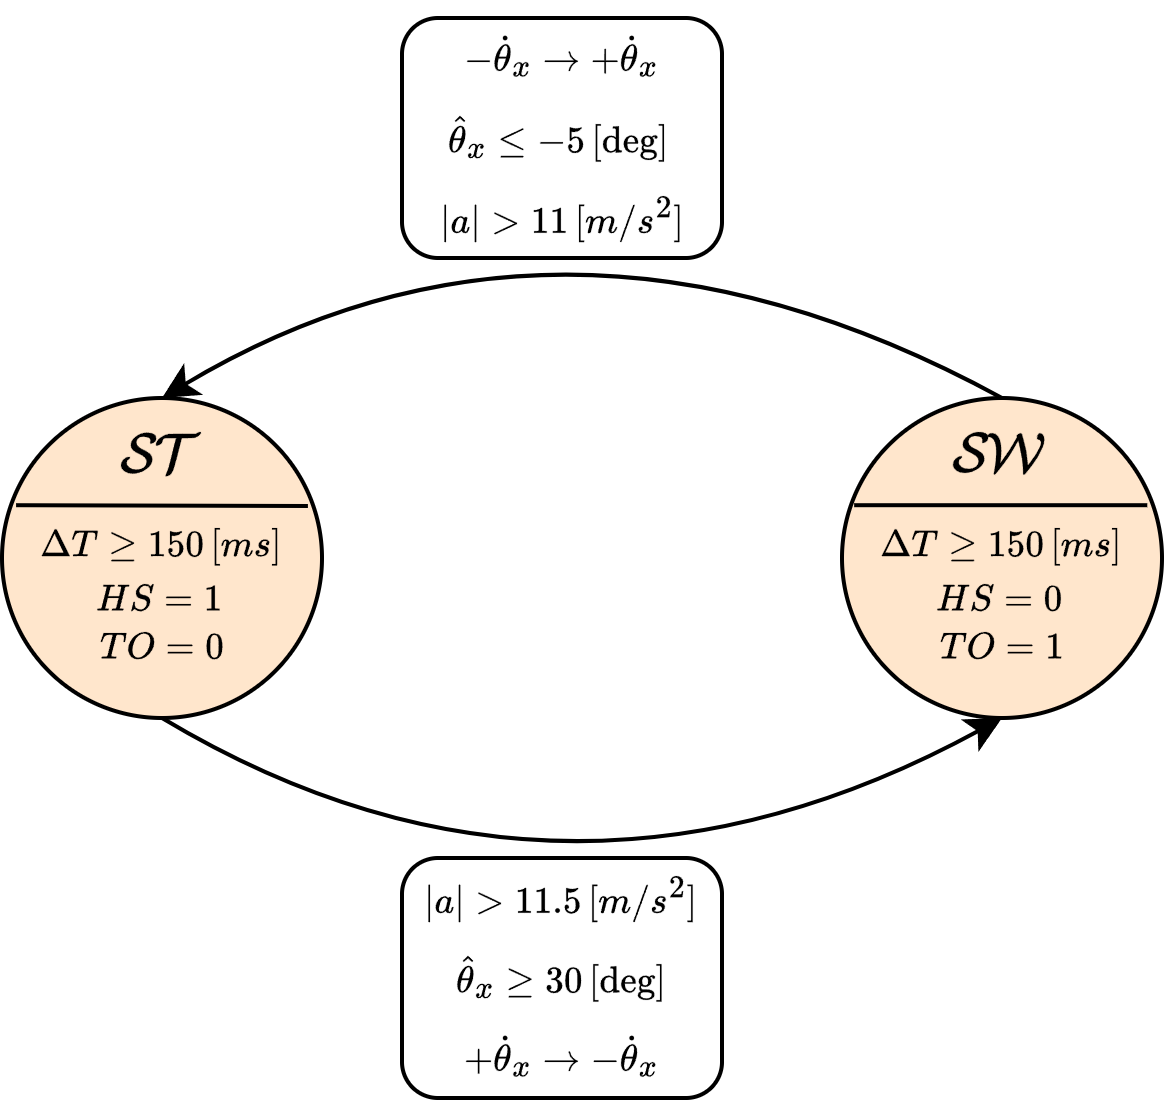
\includegraphics[width=0.5\linewidth]{stateDiagram.png}
    \caption{Gait Event Detection State Diagram}
    \label{fig:stateDiagram}
\end{figure}
Here $\hat \theta_x$ is the estimated roll angle using the complementary filter, $\dot \theta_x$ is the raw gyroscope measurement and $|a|$ is the raw magnitude measurement of all accelerometers.

\section{Drift Compensation}
The gyroscope measurement model is assumed to include white noise, and therefore when integrated (to compute relative angles) it produces random walk and drift occurs. Our focus was therefore on the angle drift compensation.
We chose to implement a complementary filter on the gyroscope and accelerometer raw data to overcome the angle drift. The filter gave an estimate of the Roll ($\phi$) and Pitch ($\theta$) Euler angles with respect to the fixed inertial frame.
First, we used the accelerometer values to calculate the direction of the gravity in an inertial frame. Then we used our previous estimation of roll and pitch to transform the raw gyroscope measurements in the body frame to the inertial frame. Finally, we applied a complementary filter using a weighting of $\alpha=95\%$ of the accelerometer estimates to compute pitch and roll. 
Regarding the estimation of the Yaw angle we concluded that based on our IMU's location on the body, gait event detection is independent of the angle's values. Thus, when performing the drift compensation we chose not to use the magnetometer.

\section{Comparison with Built in Estimation}
Our method includes estimation of two of the Euler angles with respect to a fixed inertial frame - Roll and Pitch. The drift of the third angle's (Yaw) values cannot be compensated-for using only the accelerometer and gyroscope, and requires the use of the IMU's magnetometer as well. Due to the nature of the task in measuring gait events, we concluded that we can neglect the Yaw angle estimation. Therefore, we'll compare our Roll and Pitch results to the the IMU's built-in calculations:
\begin{figure}[!h]
    \centering
    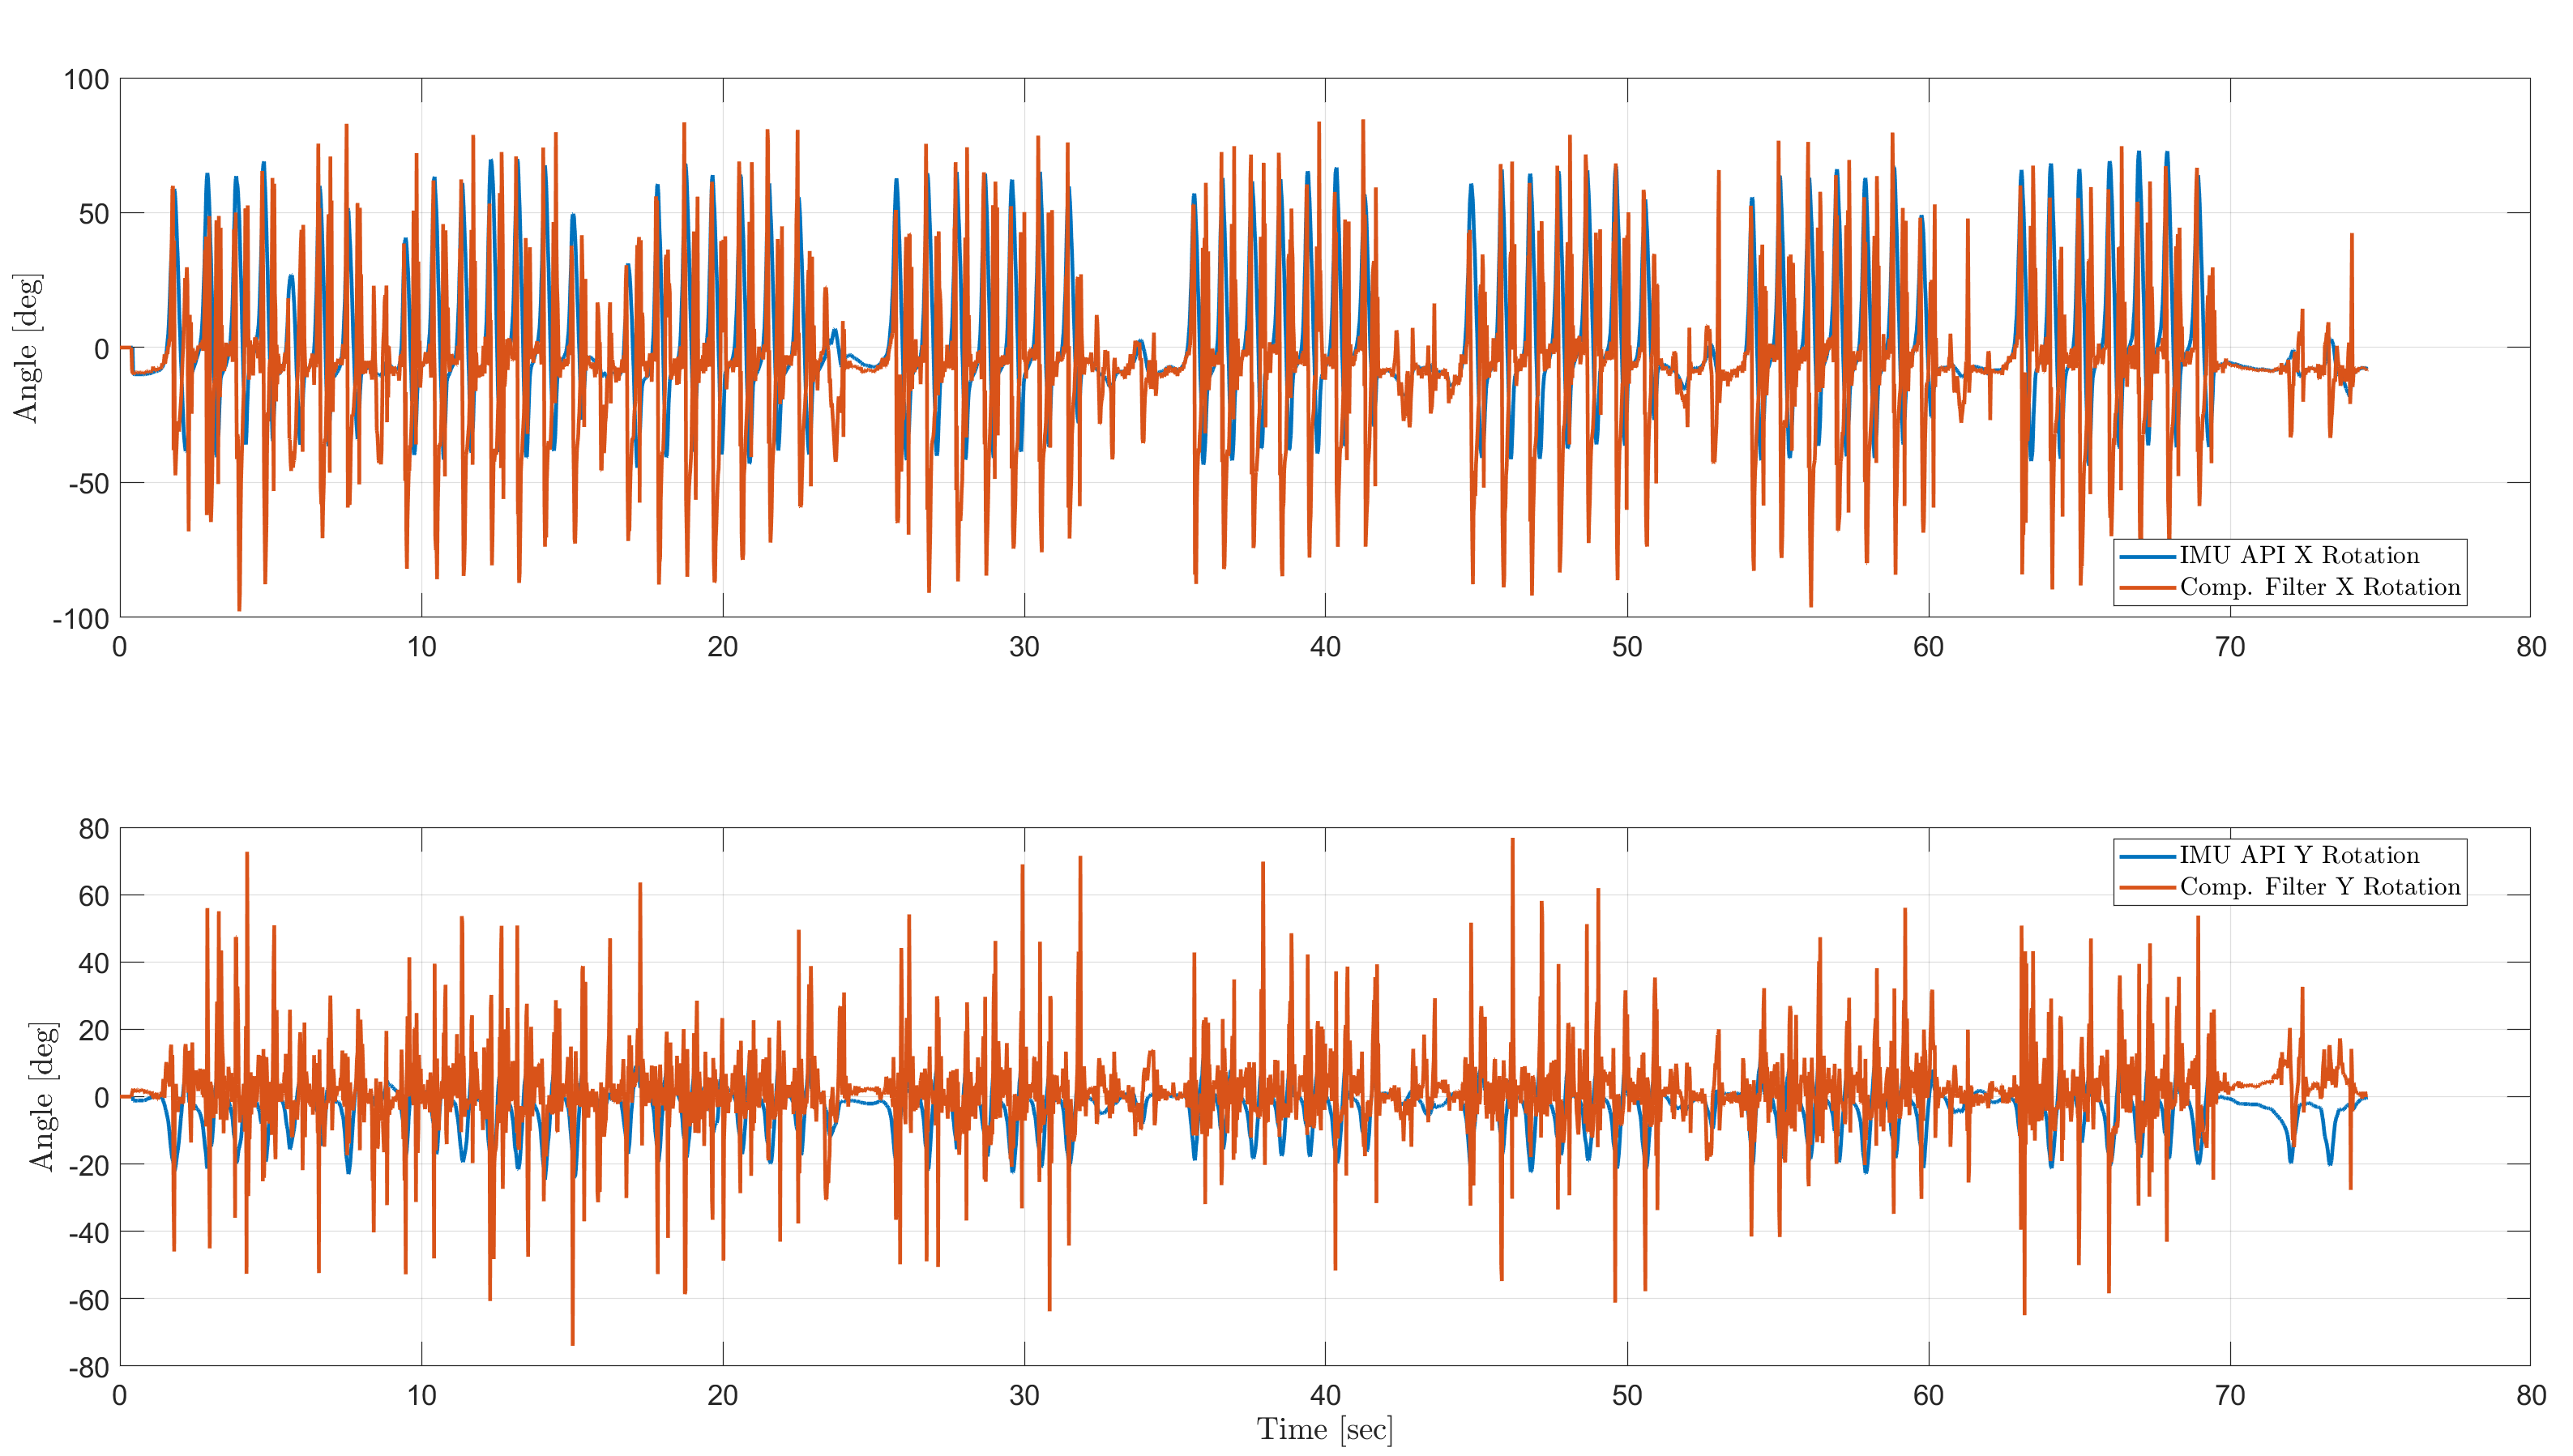
\includegraphics[width=0.75\linewidth]{image.png}
    \caption{Comparison of roll and pitch angle estimation, IMU API VS our complementary filter}
    \label{fig:imuVScomp}
\end{figure}
\begin{figure} [!h]
    \centering
    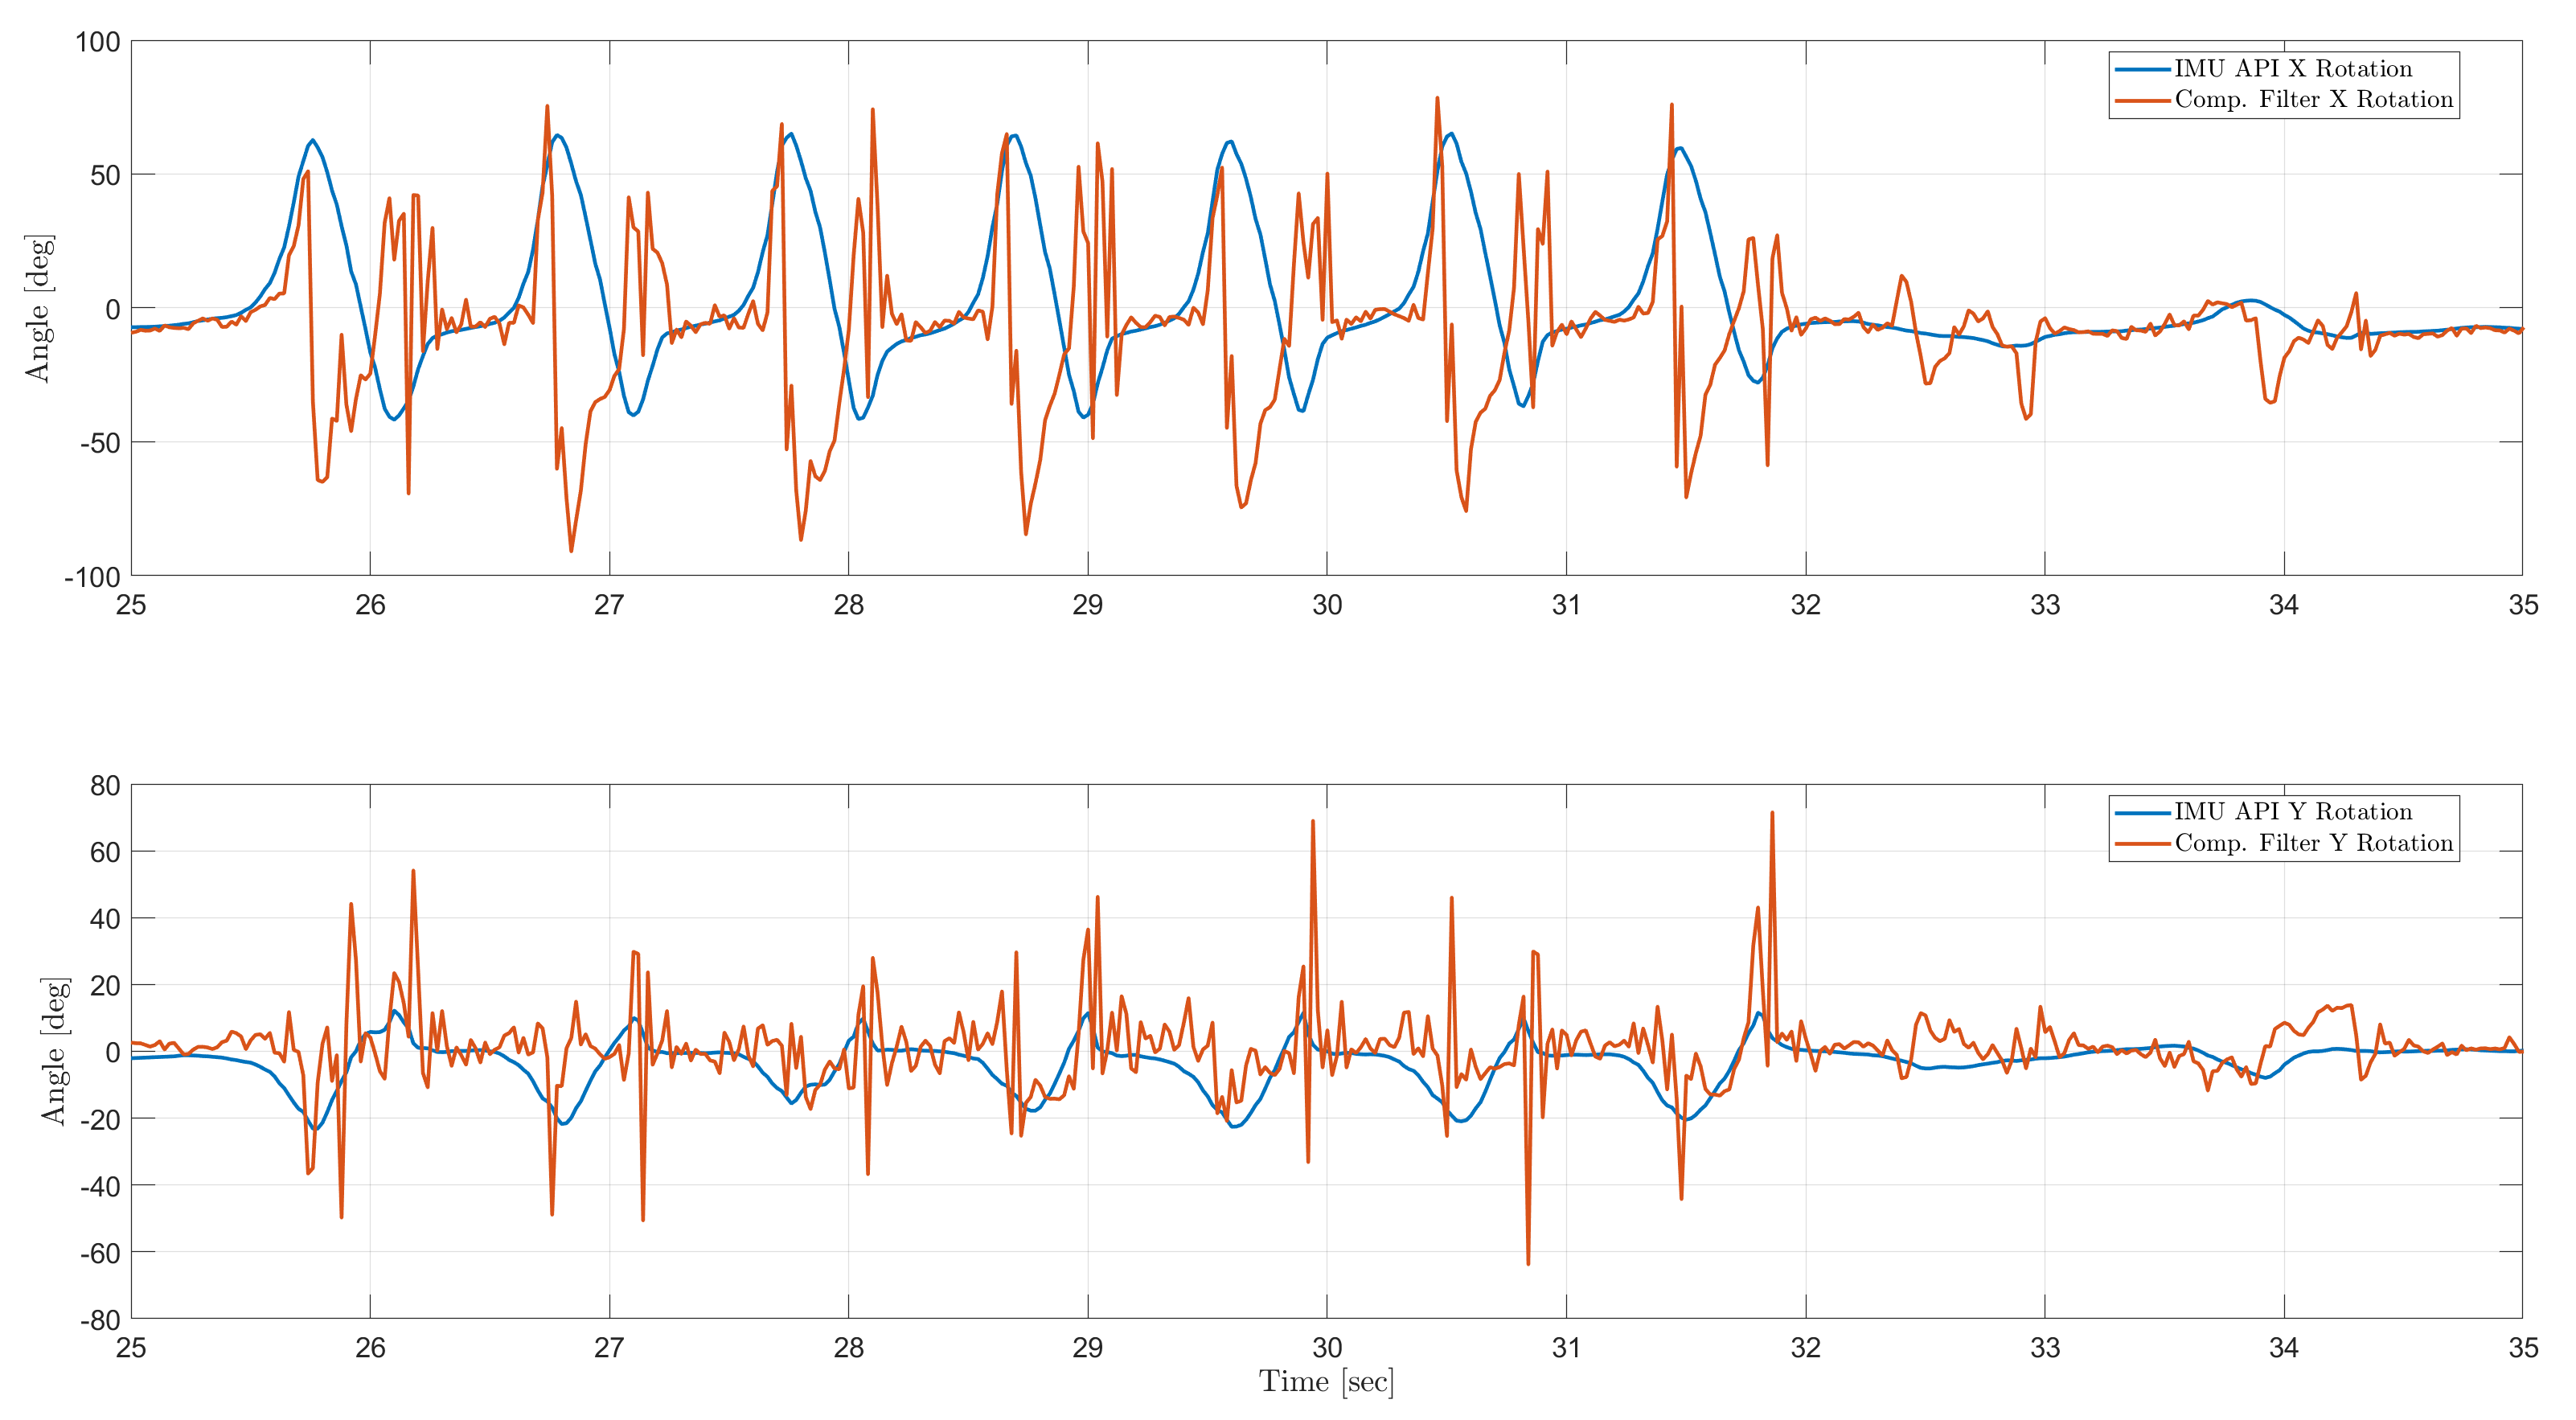
\includegraphics[width=0.75\linewidth]{image2.png}
    \caption{Zoomed 10-second snippet of figure \ref{fig:imuVScomp}}
    \label{fig:imuVScompZoom}
\end{figure}
% we need to add nice graphs
Based on the plots in figures \ref{fig:imuVScomp} and \ref{fig:imuVScompZoom} we conclude that the IMU's built-in compensation code produces better results than our complementary filter. In this case, "better results" being reduced drift and noise relative to our filter's outputs. Additionally, as the built-in methods perform their calculations using quaternions they are resistant to gimbal-lock, which is a potential issue of our implementation. As the task in this assignment doesn't require our IMU to go beyond $90^{\circ}$ or use of the Yaw angle, we don't expect this difference to prove problematic.

Due to the use of angles in our estimator, we are susceptible to gimble lock, whereas Adafruit API uses quaternion based estimation as shown in \ref{fig:gimble} 

\section{Real Time Implementation}
After we implemented our complementary filter and tested it in real-time (see the \href{https://technionmail-my.sharepoint.com/:v:/g/personal/eitangerber_campus_technion_ac_il/EU1nMidRcjNCnH50mRiva4IBxQMdXuteN7KhcMnGKk0lfQ?e=57vjzk}{linked video}), we recorded the values used in figures \ref{fig:imuVScomp} and \ref{fig:imuVScompZoom}, and additionally the acceleration magnitude and one of the states we tracked (HS - heel strike). In figure \ref{fig:states} we can see the state switching based on the acceleration and angle - it's clear that while the values themselves are mostly periodic, the state switches aren't. When watching the \href{https://technionmail-my.sharepoint.com/:v:/g/personal/eitangerber_campus_technion_ac_il/EU1nMidRcjNCnH50mRiva4IBxQMdXuteN7KhcMnGKk0lfQ?e=57vjzk}{linked video} it's clear that while the switching isn't fully accurate, for the most part the LEDs do indeed light up correctly, thus providing a visual signal for the current part of the gait cycle. Additionally, the LEDs swapping between them provides a visual signal for a gait event.

\begin{figure}[!h]
    \centering
    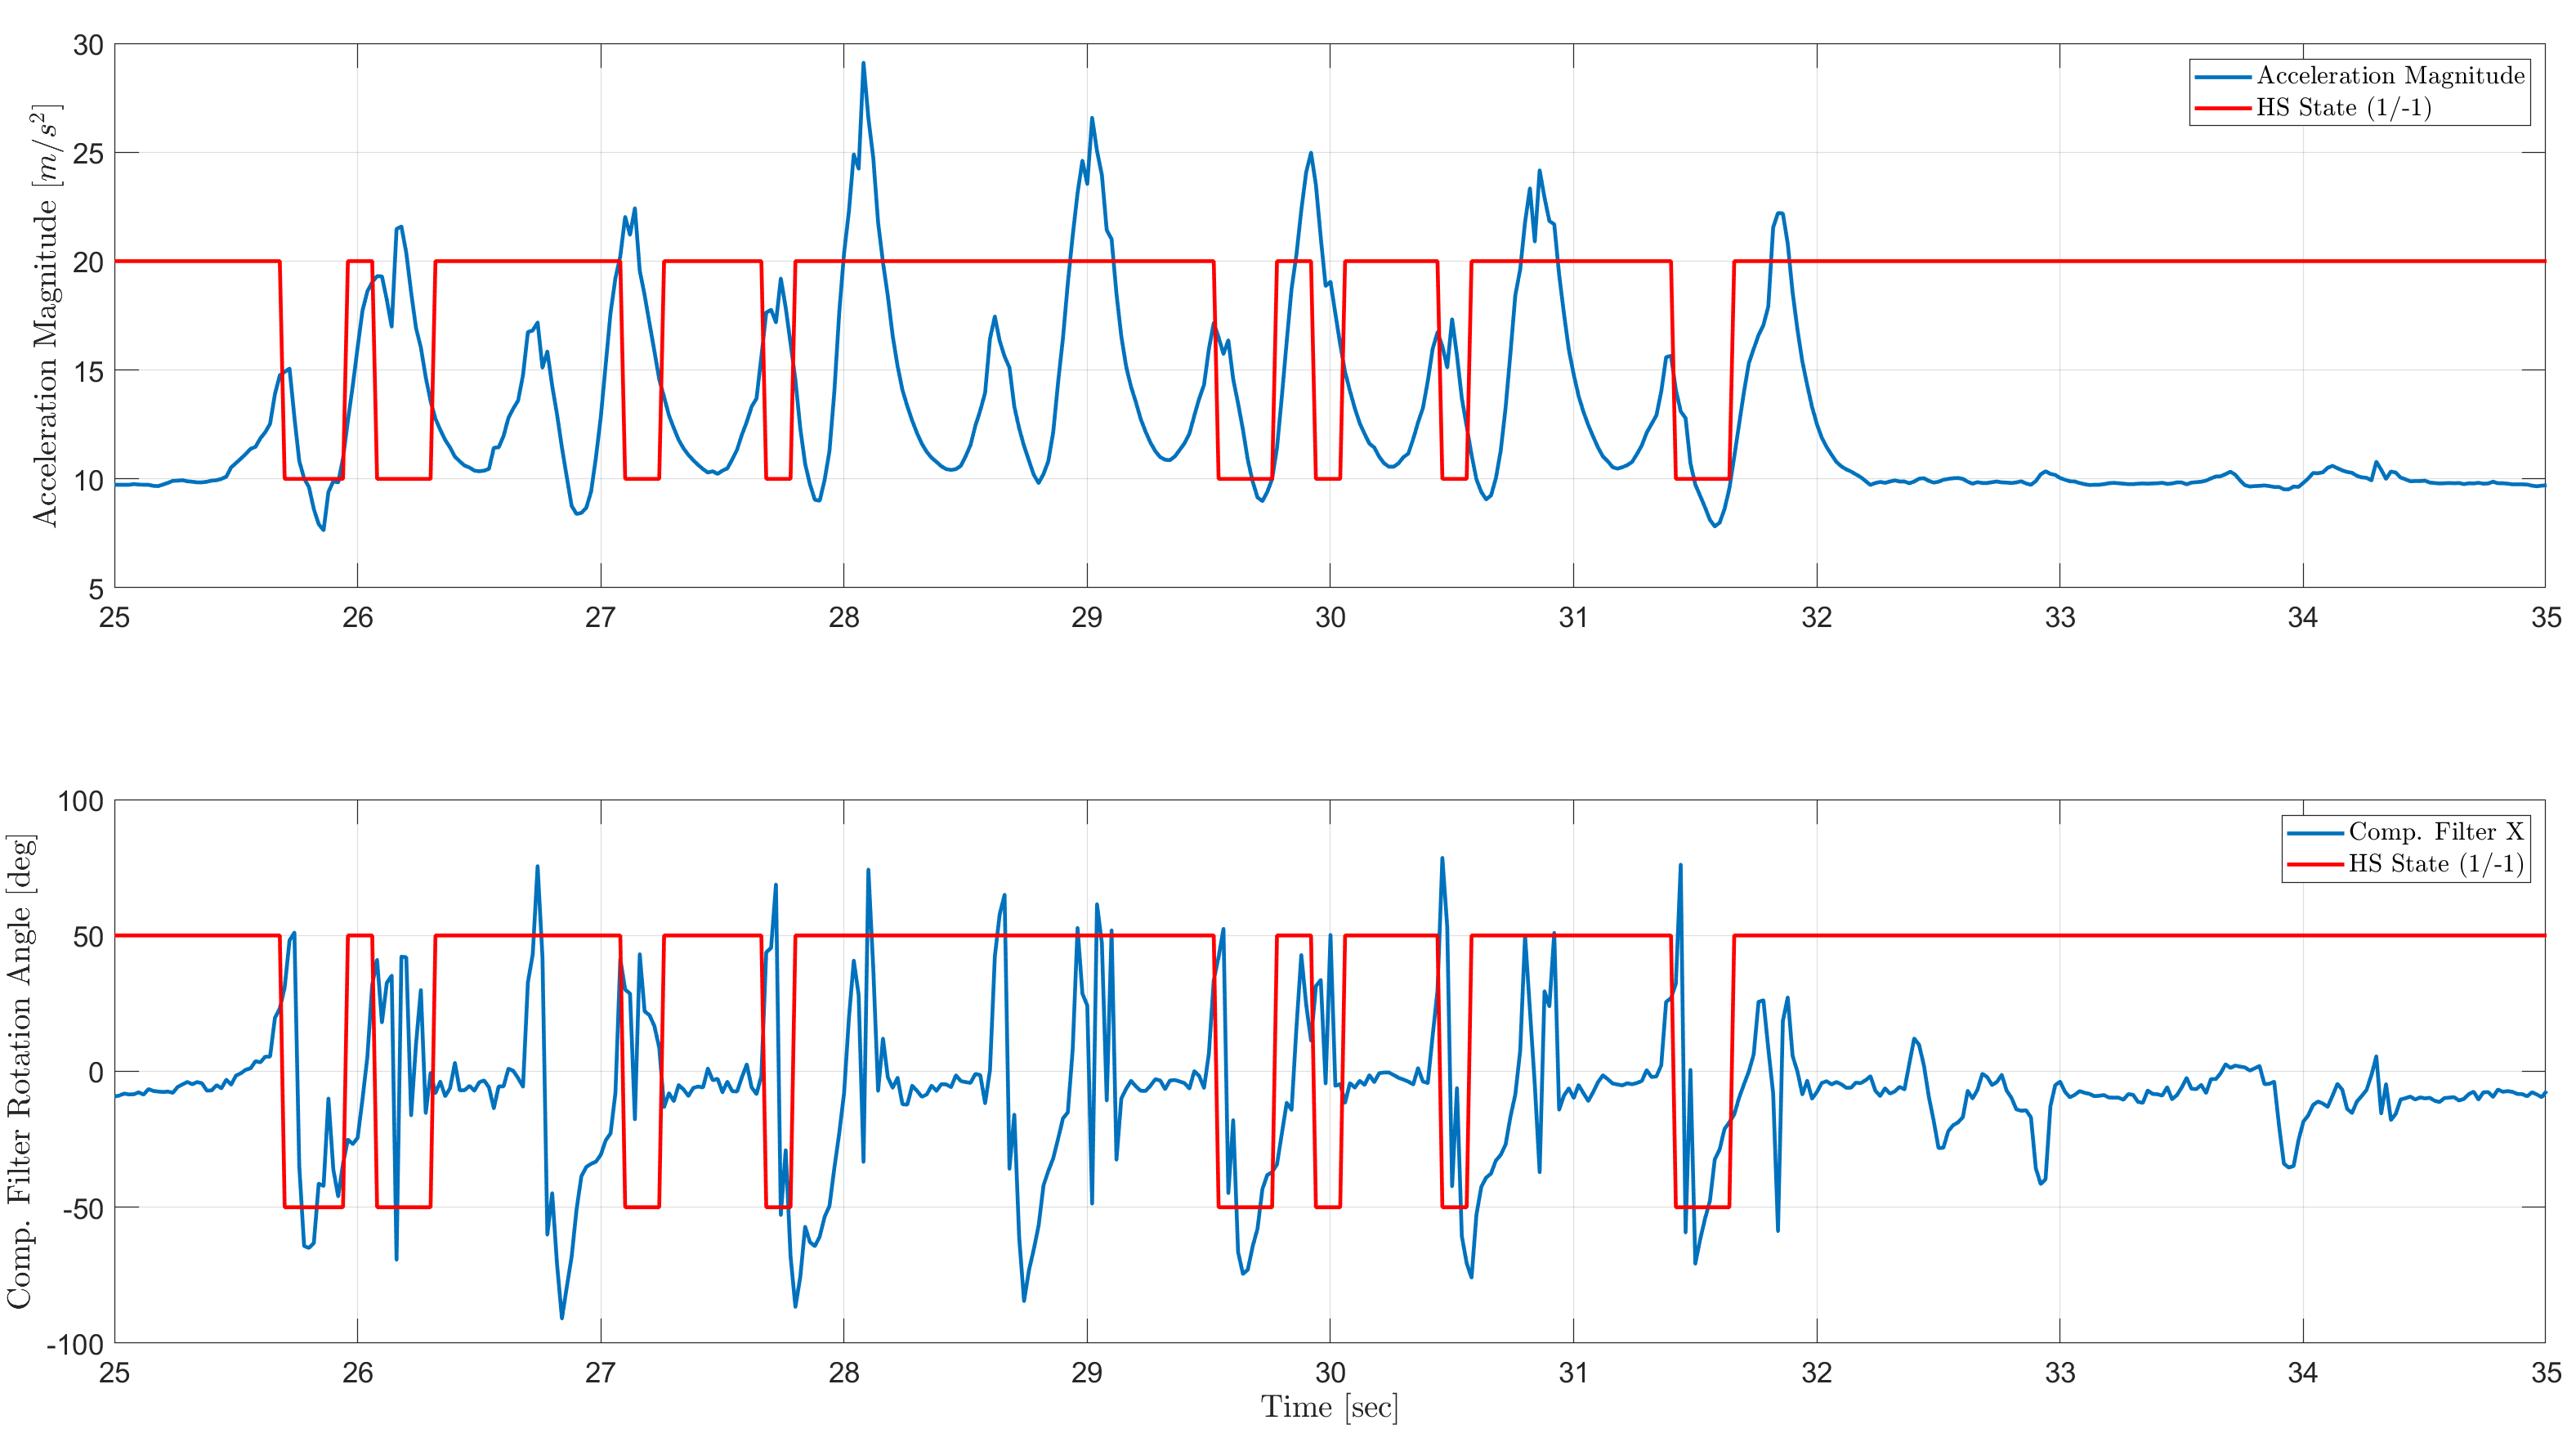
\includegraphics[width=0.75\linewidth]{imageStates.png}
    \caption{Zoomed segment of acceleration magnitude and roll angle VS the HS state. HS=1 is the stance phase (green LED), and HS=-1 is the swing phase (red LED).}
    \label{fig:states}
\end{figure}




\section{Conclusions}
Our complementary filter may not be a subject of many compliments, as it has provided unreliable angle measurement. We assume that with further tuning we may achieve a better estimator. We have learned how to implement sensor fusion on a basic level, along with a state machine, which will provide us extra tools for further research.   
% -------------------------------------- %
\end{document}